\item 

Die Höhenlinie ist die Menge aller Punkte $(x,y)$, wo die Funktion den gleichen Funktionswert besitzt, $f(x,y) = const.$ Zur Bestimmung dieser Konstanten setzen wir den Punkt $(x_0,y_0)$ ein:

$f(x,y) = f(1,2)$

$\implies e^{\frac{x^2}{y}} = e^{\frac{1}{2}}$

$\implies \frac{x^2}{y} = \frac{1}{2}$

$\implies y = 2x^2$

Die gesuchte Höhenlinie ist also eine Parabel, die um den Faktor $2$ entlang der y-Achse gestreckt ist.

Zur Bestimmung des Gradienten benötigen wir die partiellen Ableitung nach x und y:

$\frac{\partial f}{\partial x} =  \frac{2x}{y} \cdot e^{\frac{x^2}{y}}$

$\frac{\partial f}{\partial y} =  e^{\frac{x^2}{y}} \cdot (-y^{-2} \cdot x^2) = - \frac{x^2}{y^2} \cdot e^{\frac{x^2}{y}} $

Einsetzen der Höhenlinie $y=2x^2$:

$\frac{\partial f}{\partial x}|_{y=2x^2}=  e^{\frac{x^2}{2x^2}} \cdot \frac{2x}{2x^2} = e^{\frac{1}{2}}\cdot \frac{1}{x}$

$\frac{\partial f}{\partial y}|_{y=2x^2} =  -e^{\frac{x^2}{2x^2}} \cdot \frac{x^2}{4x^4} = -e^{\frac{1}{2}}\cdot \frac{1}{4x^2}$

Der Gradient auf der Höhenlinie zeigt immer in negative y-Achenrichtung (nach unten).

In der rechten Halbebene zeigt er in positive x-Richtung (nach rechts), in der linken Halbebene in negative x-Richtung (nach links).

\begin{figure}[ht]
\centering
  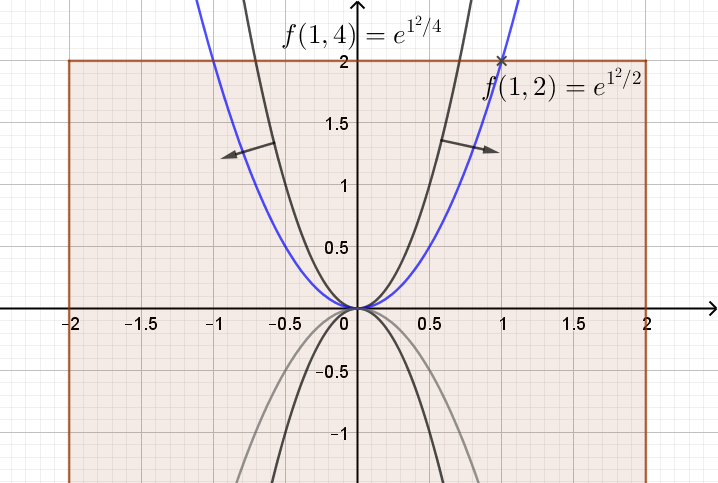
\includegraphics[width=0.4\textwidth]{../pool/ex-graph-contour-1-img-a.png}
  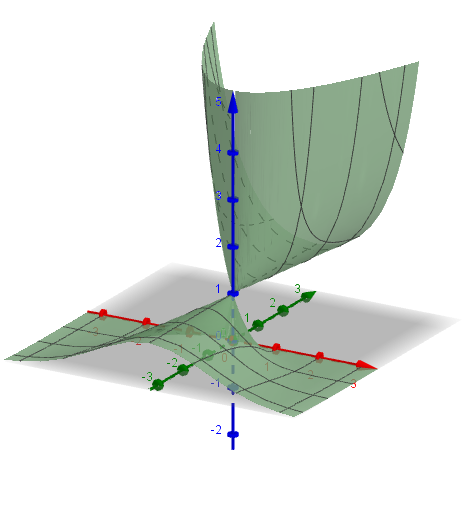
\includegraphics[width=0.4\textwidth]{../pool/ex-graph-contour-1-img-b.png}
  \caption{Höhenlinie mit Gradient zur Höhenlinie $f(x,y)=f(1,2)$ (links) und 3D-Plot davon (rechts)}
\end{figure}

